% Options for packages loaded elsewhere
\PassOptionsToPackage{unicode}{hyperref}
\PassOptionsToPackage{hyphens}{url}
%
\documentclass[
]{article}
\author{}
\date{\vspace{-2.5em}}

\usepackage{amsmath,amssymb}
\usepackage{lmodern}
\usepackage{iftex}
\ifPDFTeX
  \usepackage[T1]{fontenc}
  \usepackage[utf8]{inputenc}
  \usepackage{textcomp} % provide euro and other symbols
\else % if luatex or xetex
  \usepackage{unicode-math}
  \defaultfontfeatures{Scale=MatchLowercase}
  \defaultfontfeatures[\rmfamily]{Ligatures=TeX,Scale=1}
\fi
% Use upquote if available, for straight quotes in verbatim environments
\IfFileExists{upquote.sty}{\usepackage{upquote}}{}
\IfFileExists{microtype.sty}{% use microtype if available
  \usepackage[]{microtype}
  \UseMicrotypeSet[protrusion]{basicmath} % disable protrusion for tt fonts
}{}
\makeatletter
\@ifundefined{KOMAClassName}{% if non-KOMA class
  \IfFileExists{parskip.sty}{%
    \usepackage{parskip}
  }{% else
    \setlength{\parindent}{0pt}
    \setlength{\parskip}{6pt plus 2pt minus 1pt}}
}{% if KOMA class
  \KOMAoptions{parskip=half}}
\makeatother
\usepackage{xcolor}
\IfFileExists{xurl.sty}{\usepackage{xurl}}{} % add URL line breaks if available
\IfFileExists{bookmark.sty}{\usepackage{bookmark}}{\usepackage{hyperref}}
\hypersetup{
  hidelinks,
  pdfcreator={LaTeX via pandoc}}
\urlstyle{same} % disable monospaced font for URLs
\usepackage[margin=1in]{geometry}
\usepackage{longtable,booktabs,array}
\usepackage{calc} % for calculating minipage widths
% Correct order of tables after \paragraph or \subparagraph
\usepackage{etoolbox}
\makeatletter
\patchcmd\longtable{\par}{\if@noskipsec\mbox{}\fi\par}{}{}
\makeatother
% Allow footnotes in longtable head/foot
\IfFileExists{footnotehyper.sty}{\usepackage{footnotehyper}}{\usepackage{footnote}}
\makesavenoteenv{longtable}
\usepackage{graphicx}
\makeatletter
\def\maxwidth{\ifdim\Gin@nat@width>\linewidth\linewidth\else\Gin@nat@width\fi}
\def\maxheight{\ifdim\Gin@nat@height>\textheight\textheight\else\Gin@nat@height\fi}
\makeatother
% Scale images if necessary, so that they will not overflow the page
% margins by default, and it is still possible to overwrite the defaults
% using explicit options in \includegraphics[width, height, ...]{}
\setkeys{Gin}{width=\maxwidth,height=\maxheight,keepaspectratio}
% Set default figure placement to htbp
\makeatletter
\def\fps@figure{htbp}
\makeatother
\setlength{\emergencystretch}{3em} % prevent overfull lines
\providecommand{\tightlist}{%
  \setlength{\itemsep}{0pt}\setlength{\parskip}{0pt}}
\setcounter{secnumdepth}{-\maxdimen} % remove section numbering
\ifLuaTeX
  \usepackage{selnolig}  % disable illegal ligatures
\fi

\begin{document}

\hypertarget{predicting-the-south-african-bitcoin-ethereum-and-solana-markets-using-international-market-data}{%
\section{Predicting the South African Bitcoin, Ethereum and Solana
Markets using International Market
Data}\label{predicting-the-south-african-bitcoin-ethereum-and-solana-markets-using-international-market-data}}

\#\#1. Introduction

This paper examines the relationship between the international
cryptocurrency market and the South African cryptocurrency market. It is
hypothesized that the South African market slightly lags the
international market in terms of price movement. If this is the case and
the relationship can be modelled it could lead to improvements in
trading strategies for cryptocurrency traders. It was found that\ldots{}

This paper used data gathered from Kraken - an international
cryptocurrency exchange - to represent the international cryptocurrency
market and from VALR - a South African cryptocurrency exchange - to
represent the South African market. In specific, the per minute pricing
history for the rand and dollar markets for Bitcoin, Ethereum and Solana
were gathered from the two exchanges. Next the international markets
were compared to the local markets to test for correlation and finally
the relationships were modelled using multiple linear regressions,
gradient boosting and neural network algorithms available from
SciKit-Learn.

The paper begins by describing the data collection process before
detailing the methods of feature extraction used. Next, descriptive
statistics are presented and their implications explained following
which further data manipulation is undertaken in order to account for
the idiosyncracies of the specific dataset. Next, the methods and
results of the modelling process are presented and finally the results
are discussed in the conclusion.

\#\#2. Data Collection and Cleaning Data collection was done via email
(and WeTransfer) on the VALR side and via download on the Kraken side.
The VALR data was delivered as per minute pricing data describing the
opening-price, high-price, low-price, close-price and volume per minute.
This is known as the OHLC format. No initial cleaning was needed for the
VALR data. The VALR data was adjusted from the Pretoria, South Africa
timezone to the UTC timezone in order to match the timezone of the
Kraken data.

Kraken provides trade history for the Ethereum-USD (ETH-USD) market and
pricing history per minute for the Bitcoin-USD (BTC-USD) market in this
\href{https://drive.google.com/drive/folders/1jI3mZvrPbInNAEaIOoMbWvFfgRDZ44TT}{Google
Drive}. The ETH-USD trade history was converted into a per minute OHLC
format by grouping the trades into minute long intervals and taking the
opening trade price as the opening-price, the highest trade price as the
high-price, the lowest trade price as the low-price, the final trade
price as the closing-price and the total volume of cryptocurrency traded
as the volume.

Because the aim of this project is to use the international market for
Bitcoin and Ethereum to predict the South African market in order to
augment algorithmic trading decisions - the per minute OHCL data for
both markets was differenced by its first lag. In particular, the
closing prices were differenced and converted to a percentage. One of
the major benefits of differencing the data is that it centers it around
zero. Please see Figures 1 and 2 for a comparison of the differenced and
undifferenced BTC-USD closing prices over time. Further, differencing
(by percentage) the data brings the scale of the two markets together.
Because of the ZAR/USD exchange rate (around R15 per USD) the ZAR-BTC
and ZAR-ETH markets have nominal values around 15 times higher than the
USD markets. This is problematic if both ZAR lags and USD lags are
included in the variables input into models that work with node
weightings because it can bias the model towards variables with bigger
scales (reference here). This problem is mitigated by the scaling
inherent in differencing by percentage. After differencing, first 5 lags
of the closing prices of both the ZAR and USD markets were taken.
Similarly, a 100 period moving average and a 5 period moving average
were taken for both markets. Note that the last inclusion in the moving
averages is the first lag of the closing price.

Finally, the differenced ZAR-BTC and USD-BTC variables were divided into
8 categories dependent on the number of standard deviations that a
sample lies away from the mean. Please see Equation 1 for details.

\emph{Equation 1: Piecewise categorization of variables}

\[ Ycat=   \left\{
\begin{array}{ll}
      1 & where & \mu-2\sigma>Y \\
      2 & where & \mu-\sigma>Y>\mu-2\sigma \\
      3 & where & \mu-0,5\sigma>Y>\mu-\sigma \\
      4 & where & \mu>Y>\mu-0,5\sigma \\
      5 & where & \mu<Y<\mu+0,5\sigma \\
      6 & where & \mu+0,5\sigma<Y<\mu+\sigma \\
      7 & where & \mu+\sigma<Y<\mu+2\sigma \\
      8 & where & \mu+2\sigma<Y \\
\end{array} 
\right.  
\]

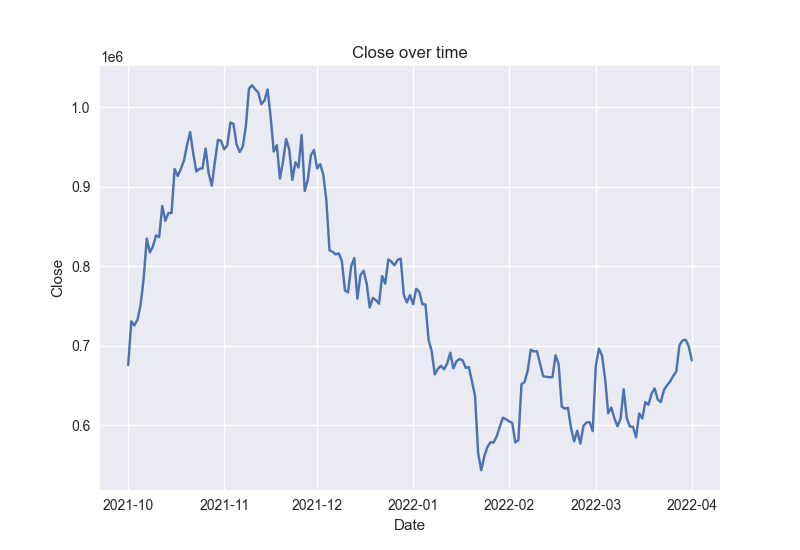
\includegraphics{/Users/pablo/Desktop/Masters/Data_Science/19119461_Data_Science_Project/Images/BTC_ZAR_vs_time.png}\\
\emph{Figure 1: BTC-ZAR over Time}

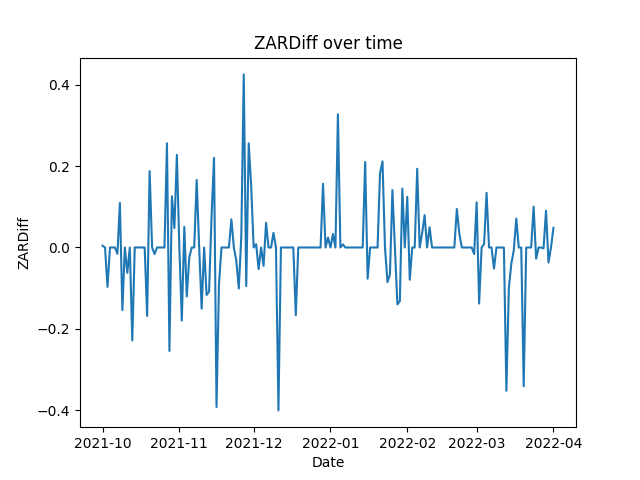
\includegraphics{/Users/pablo/Desktop/Masters/Data_Science/19119461_Data_Science_Project/Images/BTC_ZAR_Diff_vs_time.png}\\
\emph{Figure 2: Differenced BTC-ZAR over Time}

\#\#Initial analysis Single linear (OLS) regression was used to test the
hypothesis in the most basic way and a positive result was yielded.
Regressing the unlagged BTC-ZAR variable on the unlagged BTC-USD
variable reveals a strong positive relationship between the two - please
see Figure 3. Next, regressing the unlagged BTC-ZAR variable on the
first lag of the BTC-USD market yields a weaker but comparable positive
relationship - please see Figure 4. However, regressing the unlagged
BTC-USD variable on the first lag of the BTC-USD market reveals a very
weak positive relationship - please see Figure 5. Infact, even the
second lag of the BTC-USD variable is a better predictor of the unlagged
BTC-ZAR market than the first lag of the BTC-USD variable is for the
BTC-USD market. Please see Table 1 for coefficients and R-Squared
values.

\begin{longtable}[]{@{}lll@{}}
\toprule
Regression & Coefficient & R-Squared \\
\midrule
\endhead
BTC-ZARDiff on BTC-USDDiff & 0,5 & 0,17 \\
BTC-ZARDiff on BTC-USDDiff\_1 & 0,26 & 0,05 \\
BTC-USDDiff on BTC-USDDiff\_1 & 0,03 & 0,0008 \\
\bottomrule
\end{longtable}

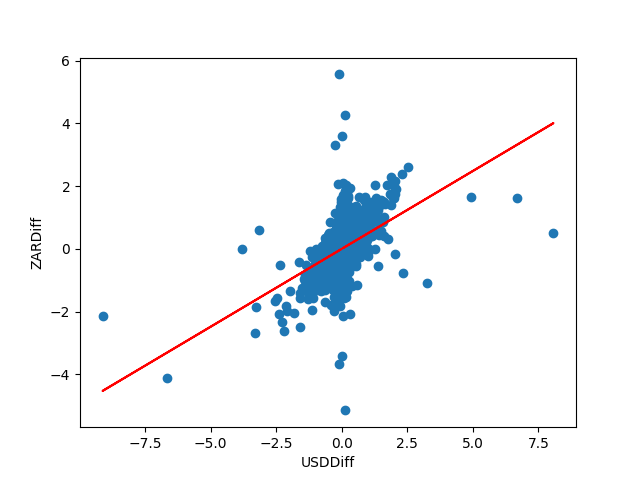
\includegraphics{/Users/pablo/Desktop/Masters/Data_Science/19119461_Data_Science_Project/Images/Scatter_ZAR_vs_USD.png}
\emph{Figure 3: Unlagged BTC-ZAR vs unlagged BTC-USD}\\
\emph{R-squared: 0.17 , Coefficient:0.5}

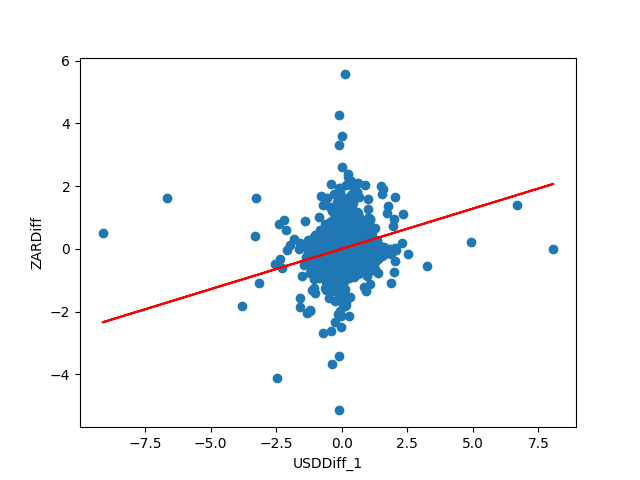
\includegraphics{/Users/pablo/Desktop/Masters/Data_Science/19119461_Data_Science_Project/Images/Scatter_ZAR_vs_USD_1.png}\\
\emph{Figure 4: First lag of BTC-ZAR vs unlagged BTC-USD}\\
\emph{R-squared: 0.05 , Coefficient:0.27}

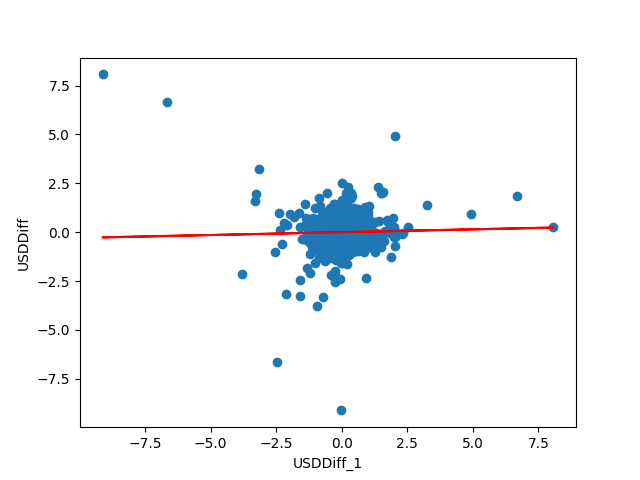
\includegraphics{/Users/pablo/Desktop/Masters/Data_Science/19119461_Data_Science_Project/Images/Scatter_USD_vs_USD_1.png}\\
\emph{Figure 5: First lag of BTC-USD vs unlagged BTC-USD}\\
\emph{R-squared: 0.0008 , Coefficient:0.03}

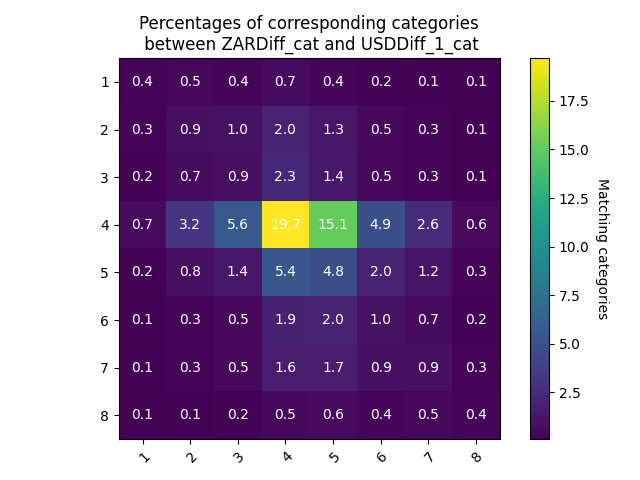
\includegraphics{/Users/pablo/Desktop/Masters/Data_Science/19119461_Data_Science_Project/Images/HMap_ZAR_vs_USD_1.png}
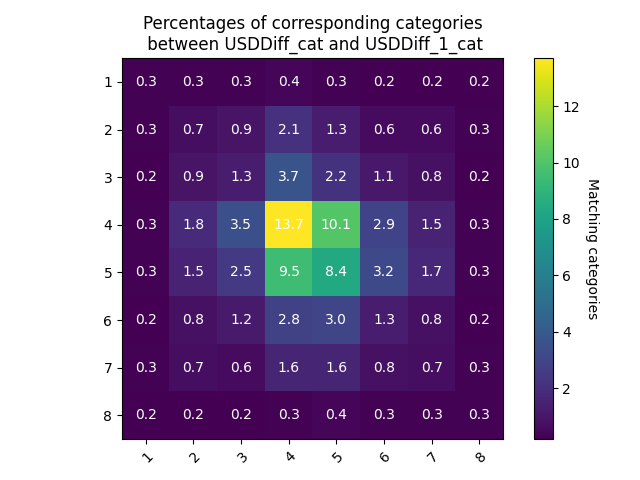
\includegraphics{/Users/pablo/Desktop/Masters/Data_Science/19119461_Data_Science_Project/Images/HMap_USD_vs_USD_1.png}

\textless-- Tables --\textgreater{}

\begin{longtable}[]{@{}ll@{}}
\toprule
Var1 & Var2 \\
\midrule
\endhead
x1 & x2 \\
x1 & x2 \\
\bottomrule
\end{longtable}

\end{document}
